\section{Experiments}
\label{chap:experiments}

\subsection{Experimental Setup}

The experiments use FB15k-237 \citep{toutanova2015observed}, which contains
14,541 entities and 237 relations. Its training, validation, and test sets
contain 272,115, 17,535, and 20,466 triples, respectively. We consider two KGE
model families, RotatE and TransE. They provide two different model settings
for checking whether the observed relation-level patterns are specific to one
embedding model.

Chapter~\ref{chap:framework} describes the comparable repeated-run setting and
the relation-level analysis design. All link-prediction results are evaluated
under the filtered setting, and
aggregate performance is reported using Hits@10. For each relation,
we report relation-level Hits@10, ambiguity ($\alpha$), and
discrepancy ($\delta$). All
relation-level figures and grouped comparisons in this chapter retain
relations with at least ten test triples
(\(\texttt{test\_support}\geq 10\)). Relation-level estimates based on very
small test support can be sensitive to a small number of query outcomes. This
threshold is therefore used to reduce the influence of such small-sample
relations on the displayed comparisons. It retains 182 relations, and unless
otherwise stated, the following analyses refer to this retained set.

\subsection{Mapping Type Analysis}
\label{sec:mapping_type_analysis}

Mapping type is the first relation-level structural factor considered in this
chapter. As defined in Chapter~\ref{chap:framework}, it categorizes a relation
according to whether its head side and tail side behave as one or many in the
training graph. The following analysis compares its four categories by
prediction side.

\subsubsection{Motivation for Side-Aware Analysis}

For a relation \(r\), tail prediction asks \((h,r,?)\), while head prediction
asks \((?,r,t)\). In the usual link-prediction evaluation, both query types are
part of the same relation-level result. A combined relation-level view therefore
computes one set of metrics for each relation after merging head-prediction and
tail-prediction queries.

This combined view is not fully aligned with how mapping type is defined.
Mapping type assigns the one-or-many property to a specific side of a relation.
For a \(1\)-\(N\) relation, the structurally many side appears in tail
prediction \((h,r,?)\): after the head entity and relation are fixed, multiple
tail entities may be plausible. The same relation does not have the same
structure on the head-prediction side \((?,r,t)\). Conversely, for an
\(M\)-\(1\) relation, the many side appears in head prediction. Therefore,
merging head and tail queries mixes the side where the mapping structure creates
more candidate ambiguity with the opposite side of the same relation.

If the two sides are combined, the result may look weaker because the difficult
side and the opposite side are averaged together. For this reason, the following
analysis reports tail prediction and head prediction separately.

\subsubsection{RotatE Results}

The RotatE results are reported separately for tail prediction and head
prediction. Each figure groups relations by mapping type and reports
relation-level Hits@10, ambiguity \(\alpha\), and discrepancy \(\delta\).
Hits@10 gives the relation-level predictive performance, while \(\alpha\) and
\(\delta\) are the two multiplicity measures used in this chapter.

\begin{figure}[!t]
    \centering
    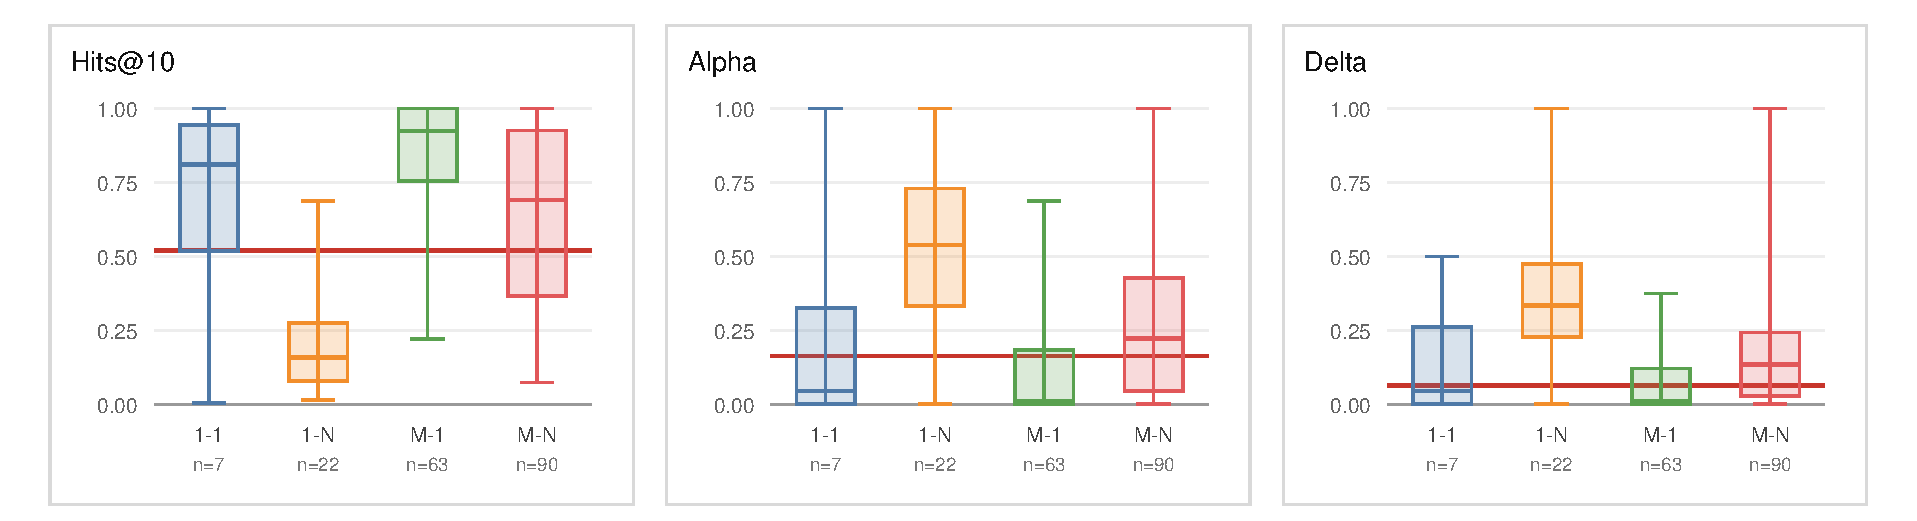
\includegraphics[width=0.86\textwidth]{figures/chap5/mapping-type/rotate-tail.pdf}
    \caption{RotatE mapping-type results for tail prediction. The red line
    marks the mean over all retained relations.}
    \label{fig:mapping-rotate-tail}
\end{figure}

The RotatE tail-prediction results are shown in
Figure~\ref{fig:mapping-rotate-tail}, which presents the clearest contrast
among the four mapping types.
The \(1\)-\(N\) group has the lowest Hits@10 and the highest
\(\alpha\) and \(\delta\). Its tail predictions are therefore less accurate and
show more hit-or-miss disagreement across the repeated RotatE runs. The
\(M\)-\(1\) group is at the other end of the comparison: it has the highest
Hits@10 and the lowest \(\alpha\) and \(\delta\). Taken together, these results
suggest that predictive multiplicity varies across mapping types in RotatE tail
prediction.

\begin{figure}[!t]
    \centering
    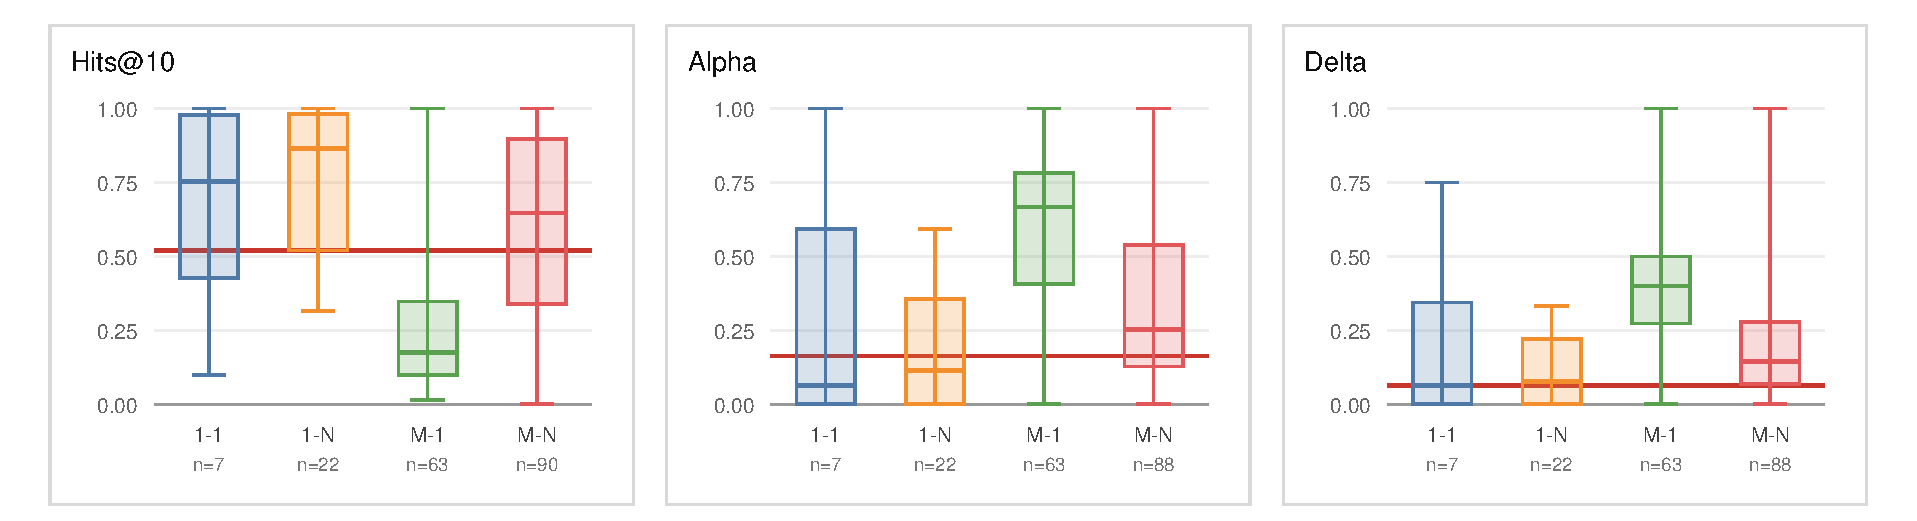
\includegraphics[width=0.86\textwidth]{figures/chap5/mapping-type/rotate-head.pdf}
    \caption{RotatE mapping-type results for head prediction. The red line
    marks the mean over all retained relations.}
    \label{fig:mapping-rotate-head}
\end{figure}

Figure~\ref{fig:mapping-rotate-head} shows a different pattern for head
prediction. The \(M\)-\(1\) group now has the lowest Hits@10 and the highest
\(\alpha\) and \(\delta\), while the \(1\)-\(N\) group has the highest Hits@10
and the lowest multiplicity measures. The relation group with lower accuracy
and higher multiplicity therefore changes when the prediction side changes.

\subsubsection{TransE Results}

The same side-aware comparison is also applied to TransE. The purpose of this
comparison is to check whether the directional pattern observed for RotatE also
appears under a different KGE model family.

\begin{figure}[!t]
    \centering
    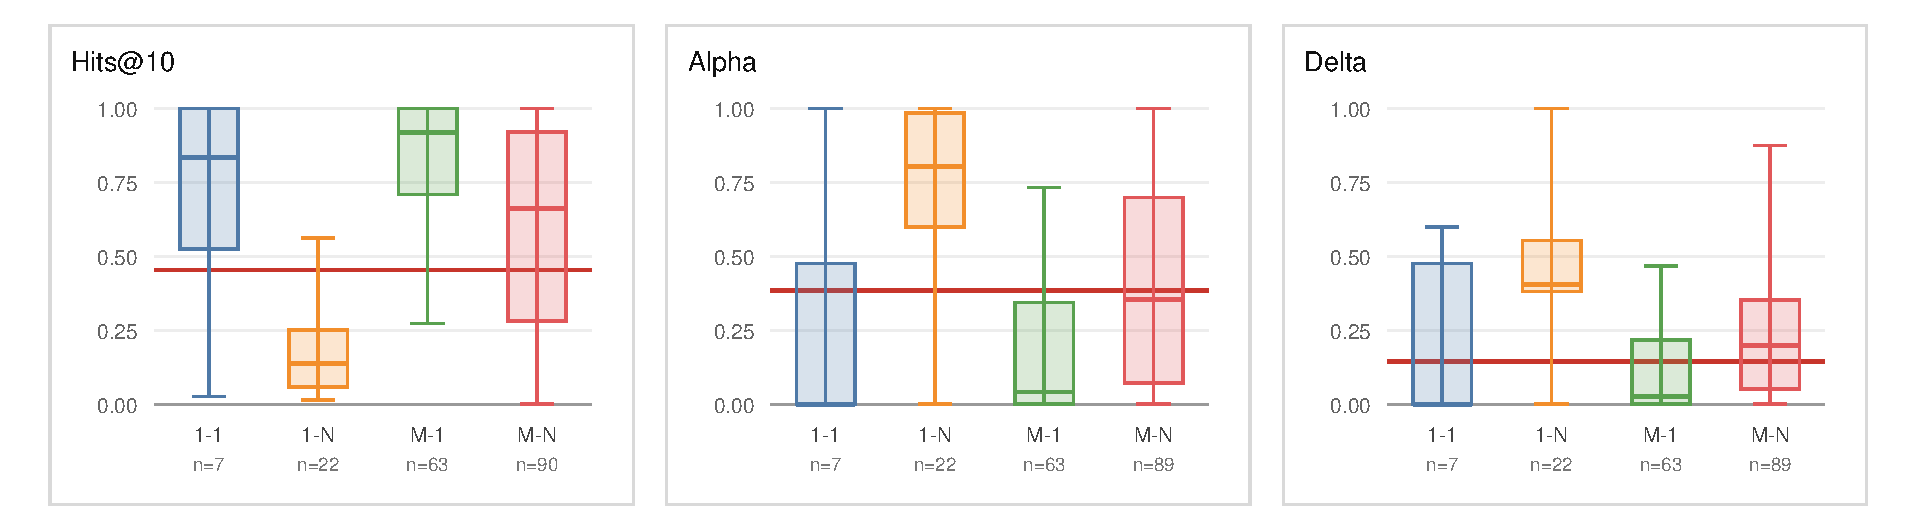
\includegraphics[width=0.86\textwidth]{figures/chap5/mapping-type/transe-tail.pdf}
    \caption{TransE mapping-type results for tail prediction. The red line
    marks the mean over all retained relations.}
    \label{fig:mapping-transe-tail}
\end{figure}

Although TransE is a different model family, its tail-prediction result shows
the same contrast between \(1\)-\(N\) and \(M\)-\(1\). In
Figure~\ref{fig:mapping-transe-tail}, the \(1\)-\(N\) group again has the
lowest Hits@10 and the highest \(\alpha\) and \(\delta\), whereas the
\(M\)-\(1\) group has the highest Hits@10 and the lowest multiplicity measures.
The lower accuracy and higher instability of the \(1\)-\(N\) tail side are
therefore observed in both models.

\begin{figure}[!t]
    \centering
    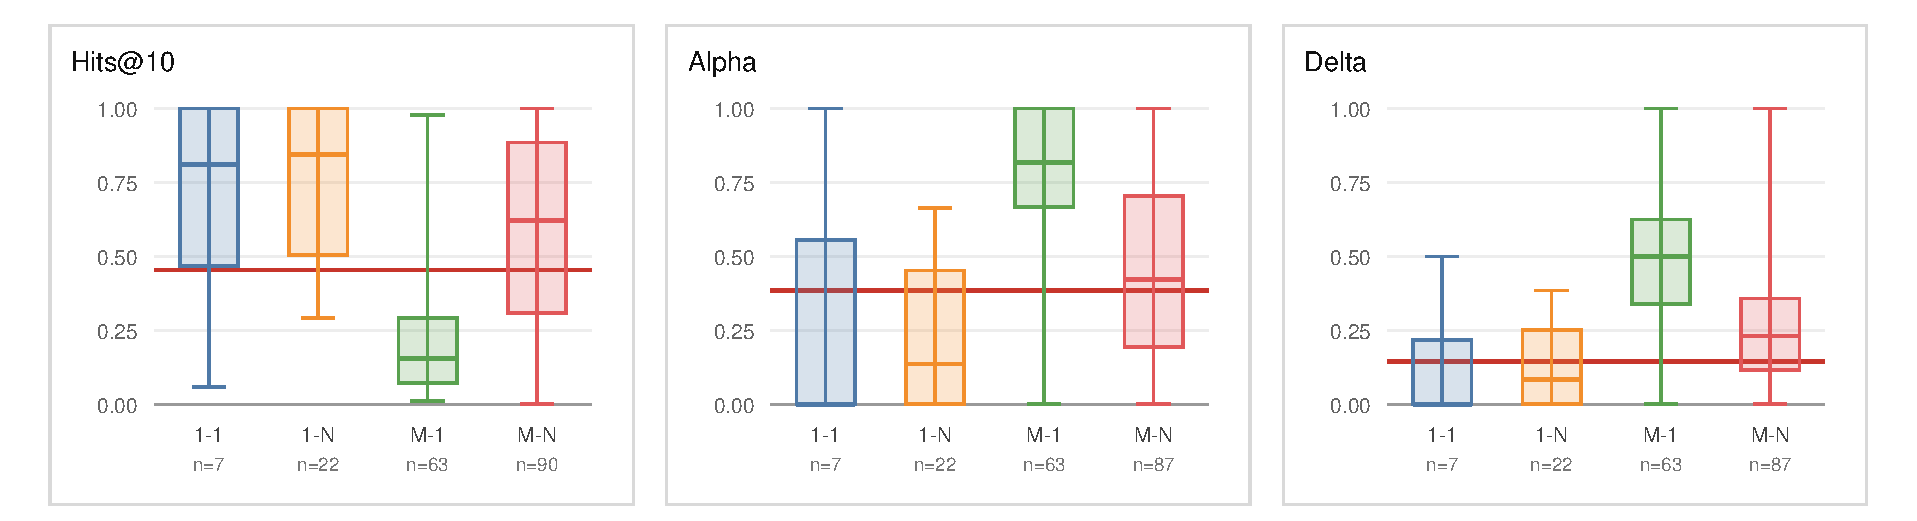
\includegraphics[width=0.86\textwidth]{figures/chap5/mapping-type/transe-head.pdf}
    \caption{TransE mapping-type results for head prediction. The red line
    marks the mean over all retained relations.}
    \label{fig:mapping-transe-head}
\end{figure}

Figure~\ref{fig:mapping-transe-head} completes the same reversal for head
prediction. The \(M\)-\(1\) group has the lowest Hits@10 and the highest
\(\alpha\) and \(\delta\). Compared with this group, the \(1\)-\(N\) group has
much higher Hits@10 and lower multiplicity measures. This agrees with the
RotatE head-prediction result.

A possible explanation is the set of constraints created by the training
triples. For a \(1\)-\(N\) relation, one fixed \((h,r)\) pair is connected to
several tail entities. Different training runs can represent or rank these
targets differently while retaining similar overall performance. This may lead
to higher \(\alpha\) and \(\delta\).

For an \(M\)-\(1\) relation, the constraints on tail prediction have a
different form. Triples such as \((h_1,r,t)\), \((h_2,r,t)\), and
\((h_3,r,t)\) provide several training constraints involving the same tail
entity, but each constraint belongs to a different tail query. The many-valued
structure is therefore on the head side rather than on the predicted tail side.
The same reasoning applies in reverse to head prediction, where a fixed
\((r,t)\) pair in an \(M\)-\(1\) relation is connected to multiple possible
head entities.

Under filtered evaluation, other known true answers are removed before the
candidate ranking is evaluated. The observed difference is therefore not
simply caused by known answers competing directly in the candidate list. The
four figures suggest that the constraints learned from the many side of
a relation leave more room for repeated runs to produce different ranking
decisions. This interpretation is consistent with the observed results, but
the current experiment does not test this training mechanism separately.

Overall, RotatE and TransE show the same side-dependent pattern on FB15k-237.
For \(1\)-\(N\) and \(M\)-\(1\) relations, predicting the side classified as
many is associated with lower accuracy and higher predictive multiplicity than
predicting the opposite side. This result suggests that the relation between
mapping type and predictive multiplicity depends on which side is predicted.

Tables~\ref{tab:mapping-type-tail-summary}
and~\ref{tab:mapping-type-head-summary} report the corresponding grouped means
for tail and head prediction.

\begin{table}[!t]
    \centering
    \caption{Relation-level means for tail prediction under
    \(\texttt{test\_support}\geq 10\).}
    \label{tab:mapping-type-tail-summary}
    \small
    \begin{tabular}{llrrr}
        \toprule
        Model & Mapping type & Hits@10 & \(\alpha\) & \(\delta\) \\
        \midrule
        RotatE & \(1\)-\(1\) & 0.6771 & 0.2422 & 0.1529 \\
        RotatE & \(1\)-\(N\) & 0.2104 & 0.5234 & 0.3659 \\
        RotatE & \(M\)-\(1\) & 0.8251 & 0.1076 & 0.0731 \\
        RotatE & \(M\)-\(N\) & 0.6313 & 0.2646 & 0.1591 \\
        TransE & \(1\)-\(1\) & 0.7016 & 0.2790 & 0.2218 \\
        TransE & \(1\)-\(N\) & 0.1741 & 0.7147 & 0.4596 \\
        TransE & \(M\)-\(1\) & 0.8180 & 0.1809 & 0.1117 \\
        TransE & \(M\)-\(N\) & 0.6065 & 0.3877 & 0.2200 \\
        \bottomrule
    \end{tabular}
\end{table}

\begin{table}[!t]
    \centering
    \caption{Relation-level means for head prediction under
    \(\texttt{test\_support}\geq 10\).}
    \label{tab:mapping-type-head-summary}
    \small
    \begin{tabular}{llrrr}
        \toprule
        Model & Mapping type & Hits@10 & \(\alpha\) & \(\delta\) \\
        \midrule
        RotatE & \(1\)-\(1\) & 0.6664 & 0.3216 & 0.2145 \\
        RotatE & \(1\)-\(N\) & 0.7527 & 0.1939 & 0.1168 \\
        RotatE & \(M\)-\(1\) & 0.2836 & 0.5855 & 0.3835 \\
        RotatE & \(M\)-\(N\) & 0.5971 & 0.3366 & 0.1994 \\
        TransE & \(1\)-\(1\) & 0.6861 & 0.3015 & 0.1332 \\
        TransE & \(1\)-\(N\) & 0.7455 & 0.2261 & 0.1339 \\
        TransE & \(M\)-\(1\) & 0.2439 & 0.7523 & 0.4893 \\
        TransE & \(M\)-\(N\) & 0.5764 & 0.4355 & 0.2474 \\
        \bottomrule
    \end{tabular}
\end{table}

\subsection{Inverse Relation Analysis}
\label{sec:inverse_analysis}

\subsubsection{Motivation}

When two relations form an inverse pair, they describe the connection between
the same entities in opposite directions. Training edges under the two
relations can therefore provide paired structural evidence: one relation
supports the connection from the head to the tail, while its inverse partner
supports the reversed connection. Such evidence may constrain the relation
representations learned under different random seeds and make their ranking
decisions more stable.

The analysis uses the inverse clarity defined in
Chapter~\ref{chap:framework}. This score measures whether the strongest mutual
inverse partner of a relation is clearly separated from its second-best
partner. A high value therefore indicates both substantial reverse support and
a clearly identified inverse partner. For readability, the tables in this
section use \emph{score} as a shorter name for inverse clarity.

\subsubsection{Results}

Table~\ref{tab:inverse-spearman} reports the global Spearman correlations
between the inverse score and the three relation-level evaluation metrics.
Across all relations, the inverse score does not show a monotonic association
with improved accuracy or stability. For RotatE and TransE, the Spearman
correlations with Hits@10 are \(-0.2796\) and \(-0.2819\), respectively. The
corresponding correlations with \(\alpha\) and \(\delta\) are positive and
range from \(0.2263\) to \(0.2427\). These global correlations therefore do
not indicate a general accuracy or stability benefit as the inverse score
increases.

\begin{table}[!t]
    \centering
    \caption{Spearman correlations between inverse clarity and relation-level
    Hits@10, \(\alpha\), and \(\delta\).}
    \label{tab:inverse-spearman}
    \small
    \begin{tabular}{lrrr}
        \toprule
        Model & Spearman (Hits@10) & Spearman (\(\alpha\)) &
        Spearman (\(\delta\)) \\
        \midrule
        RotatE & -0.2796 & 0.2398 & 0.2263 \\
        TransE & -0.2819 & 0.2371 & 0.2427 \\
        \bottomrule
    \end{tabular}
\end{table}

The global correlations do not show a monotonic benefit across all relations.
However, the score-group comparison in
Table~\ref{tab:inverse-score-groups} reveals a distinct pattern at the upper
end of the inverse-score distribution. The five relations with scores above
\(0.5\) show the clearest positive result. For RotatE, mean Hits@10 reaches
\(0.8000\), compared with \(0.5797\) across all retained relations, while both
\(\alpha\) and \(\delta\) fall to \(0\). For TransE, mean Hits@10 reaches
\(0.6866\), compared with the overall mean of \(0.5585\), while \(\alpha\) and
\(\delta\) decrease from the overall means of \(0.3357\) and \(0.1885\) to
\(0.1361\) and \(0.0813\), respectively. In the current experiment, relations
with a strong and clearly identified inverse partner are therefore associated
with higher accuracy and substantially lower predictive multiplicity in both
models. The lower score ranges do not show a gradual improvement: relations in
\((0,0.5]\) have lower Hits@10 and higher multiplicity than those with a score
of zero.

\begin{table}[!t]
    \centering
    \caption{Relation-level results grouped by inverse clarity. The label
    \emph{Score} in the table refers to the inverse clarity defined in
    Chapter~\ref{chap:framework}.}
    \label{tab:inverse-score-groups}
    \small
    \begin{tabular}{llrrrr}
        \toprule
        Model & Score range & Relations & Hits@10 & \(\alpha\) & \(\delta\) \\
        \midrule
        RotatE & All relations & 182 & 0.5797 & 0.2433 & 0.1427 \\
        \cmidrule(lr){1-6}
        RotatE & Score \(=0\) & 78 & 0.6700 & 0.1721 & 0.1031 \\
        RotatE & \(0<\text{Score}\leq 0.5\) & 99 & 0.4974 & 0.3116 & 0.1812 \\
        RotatE & Score \(>0.5\) & 5 & 0.8000 & 0.0000 & 0.0000 \\
        \midrule
        TransE & All relations & 182 & 0.5585 & 0.3357 & 0.1885 \\
        \cmidrule(lr){1-6}
        TransE & Score \(=0\) & 78 & 0.6480 & 0.2565 & 0.1452 \\
        TransE & \(0<\text{Score}\leq 0.5\) & 99 & 0.4816 & 0.4082 & 0.2281 \\
        TransE & Score \(>0.5\) & 5 & 0.6866 & 0.1361 & 0.0813 \\
        \bottomrule
    \end{tabular}
\end{table}

One possible interpretation is that partial or ambiguous reverse support is
not sufficient to provide a consistent paired constraint. When the inverse
score is high, the reverse evidence is concentrated on a strong and clearly
separated partner, which may reduce variation across repeated runs. Although
the high-score range contains only five relations, the same pattern of higher
accuracy and lower predictive multiplicity appears in both RotatE and TransE.

\subsection{Symmetry Analysis}
\label{sec:symmetry_analysis}

\subsubsection{Motivation}

For a symmetric relation, an entity pair can be connected by the same relation
in both directions. The two endpoint entities can therefore occupy compatible
roles under that relation, and the training graph provides structural evidence
for both directional orderings. This may reduce the distinction between the
head and tail roles and make predictions less sensitive to differences between
repeated runs.

As discussed in Chapter~\ref{chap:framework}, the raw symmetry score can be
inflated by self-loop triples because a self-loop is identical to its reversed
edge. The following analysis therefore uses the symmetry score that excludes
self-loops, \(\operatorname{Sym}^{\neg\mathrm{loop}}(r)\). The shorter label
\emph{Score} in the tables refers to this excluding-self-loop score.

\subsubsection{Results}

The global correlations in Table~\ref{tab:symmetry-spearman} do not show a
clear monotonic association. For both models, the correlation between the
excluding-self-loop symmetry score and Hits@10 is close to zero. The
correlations with \(\alpha\) and \(\delta\) are also weak. Thus, the symmetry
score does not provide a global explanation of either predictive performance or
multiplicity.

\begin{table}[!t]
    \centering
    \caption{Spearman correlations between the excluding-self-loop symmetry
    score and relation-level Hits@10, \(\alpha\), and \(\delta\).}
    \label{tab:symmetry-spearman}
    \small
    \begin{tabular}{lrrr}
        \toprule
        Model & Spearman (Hits@10) & Spearman (\(\alpha\)) &
        Spearman (\(\delta\)) \\
        \midrule
        RotatE & 0.0122 & 0.1310 & 0.1292 \\
        TransE & 0.0117 & 0.0425 & 0.0520 \\
        \bottomrule
    \end{tabular}
\end{table}

In Table~\ref{tab:symmetry-score-groups}, Hits@10 falls in the middle score
range and returns to slightly above the zero-score level in the high-score
range for both models. The multiplicity results are less consistent. In the
high-score range, both \(\alpha\) and \(\delta\) remain higher than those of the
zero-score relations. From the middle to the high-score range, they increase
slightly for RotatE but decrease for TransE. Higher symmetry scores are
therefore not consistently associated with lower predictive multiplicity.

\begin{table}[!t]
    \centering
    \caption{Relation-level results grouped by the excluding-self-loop
    symmetry score.}
    \label{tab:symmetry-score-groups}
    \small
    \begin{tabular}{llrrrr}
        \toprule
        Model & Score range & Relations & Hits@10 & \(\alpha\) & \(\delta\) \\
        \midrule
        RotatE & All relations & 182 & 0.5797 & 0.2433 & 0.1427 \\
        \cmidrule(lr){1-6}
        RotatE & Score \(=0\) & 164 & 0.5815 & 0.2294 & 0.1331 \\
        RotatE & \(0<\text{Score}\leq 0.5\) & 6 & 0.5047 & 0.3610 & 0.2236 \\
        RotatE & Score \(>0.5\) & 12 & 0.5924 & 0.3735 & 0.2341 \\
        \midrule
        TransE & All relations & 182 & 0.5585 & 0.3357 & 0.1885 \\
        \cmidrule(lr){1-6}
        TransE & Score \(=0\) & 164 & 0.5605 & 0.3307 & 0.1838 \\
        TransE & \(0<\text{Score}\leq 0.5\) & 6 & 0.4725 & 0.4436 & 0.2736 \\
        TransE & Score \(>0.5\) & 12 & 0.5742 & 0.3512 & 0.2119 \\
        \bottomrule
    \end{tabular}
\end{table}

A possible explanation is that symmetry places only a broad constraint on the
answer space. If a relation often appears in both directions, the entities on
its two sides are likely to have similar semantic roles. This may help the
model rule out clearly unsuitable candidates and may explain the slightly
higher Hits@10 in the high-score range. Symmetry still does not distinguish
among candidates that fit the same broad constraint. Different runs may still
rank these candidates differently, which may explain why \(\alpha\) and
\(\delta\) in the high-score range remain above those of the zero-score
relations. However, this explanation does not account for the lower Hits@10 in
the six-relation middle range, which remains unclear.
